% Requires \usepackage{graphicx} in the paper preamble.
% Paths are relative to the paper's main .tex file.
\begin{figure}[t]
  \centering
  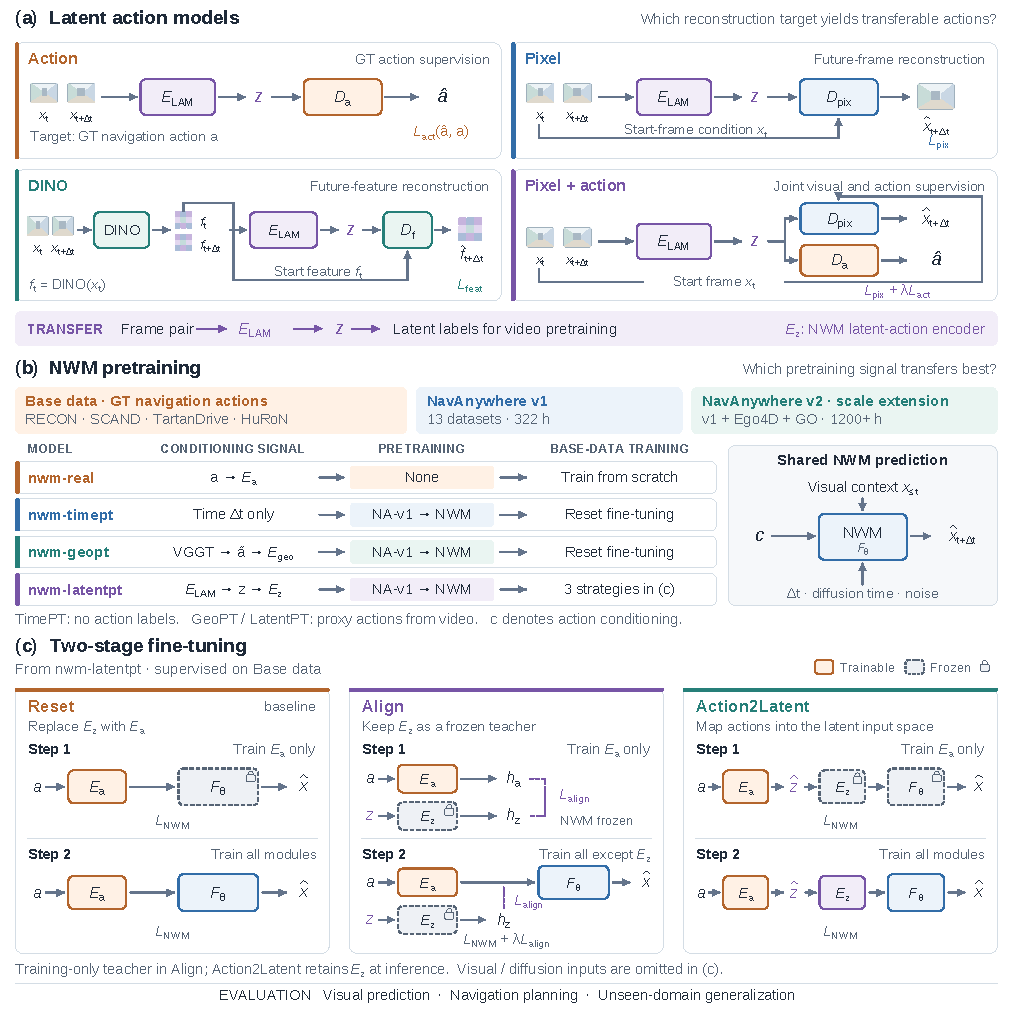
\includegraphics[width=\textwidth]{figures/lam_nwm/overview.pdf}
  \caption{\textbf{Design choices for transferable latent actions and navigation world models.}
  \textbf{(a) LAM objectives.} A frame-pair encoder $E_{\mathrm{LAM}}$ produces a latent action $z$.
  Action only reconstructs the ground-truth navigation action; Pixel reconstructs the future frame from $z$ and the initial frame; DINO encodes both frames into features and reconstructs future features from $z$ and initial-frame features; Pixel + action combines pixel and action reconstruction.
  \textbf{(b) NWM pretraining.} NWM-Real trains directly on action-labeled Base data.
  TimePT, GeoPT, and LatentPT pretrain on NavAnywhere using time conditioning without action labels, VGGT-derived geometric actions, and LAM-derived latent actions, respectively, before adaptation on Base data.
  NavAnywhere v2 extends v1 with Ego4D and GO to study data scale.
  Base data comprises RECON, SCAND, TartanDrive, and HuRoN; the LAM experiments train on RECON, SCAND, and HuRoN, holding out TartanDrive for out-of-domain evaluation.
  \textbf{(c) Two-step fine-tuning of LatentPT.} $E_z$ maps latent actions to NWM conditioning embeddings and is distinct from $E_{\mathrm{LAM}}$.
  Reset replaces $E_z$ with $E_a$; Align matches $E_a(a)$ to a frozen $E_z(z)$ teacher; Action2Latent uses $E_z(E_a(a))$.
  Step 1 trains only $E_a$: Reset and Action2Latent use the NWM objective, while Align uses embedding alignment.
  Step 2 jointly trains the active NWM path; Align retains its frozen teacher and alignment objective, whereas Action2Latent also updates $E_z$.
  All three inference paths condition on real actions without requiring future frames or the LAM extractor.
  Loss symbols denote training objectives without specifying their implementation or weights.}
  \label{fig:lam-nwm-design}
\end{figure}
